\section{Where CIF is weaker}
\label{app:weaker}

\Cref{fig:high-p-boundary} shows, by downstream learner, where the
classification scores of CIF peak on the 15 datasets with more than 100
features, the pattern summarized in \cref{sec:boundary}. Scores peak at
intermediate $k$ ($100<k<p$) on 8 of 15 LR datasets, 12 of 15 SVM datasets, and
9 of 15 KNN datasets.

\begin{figure}[tb]
  \centering
  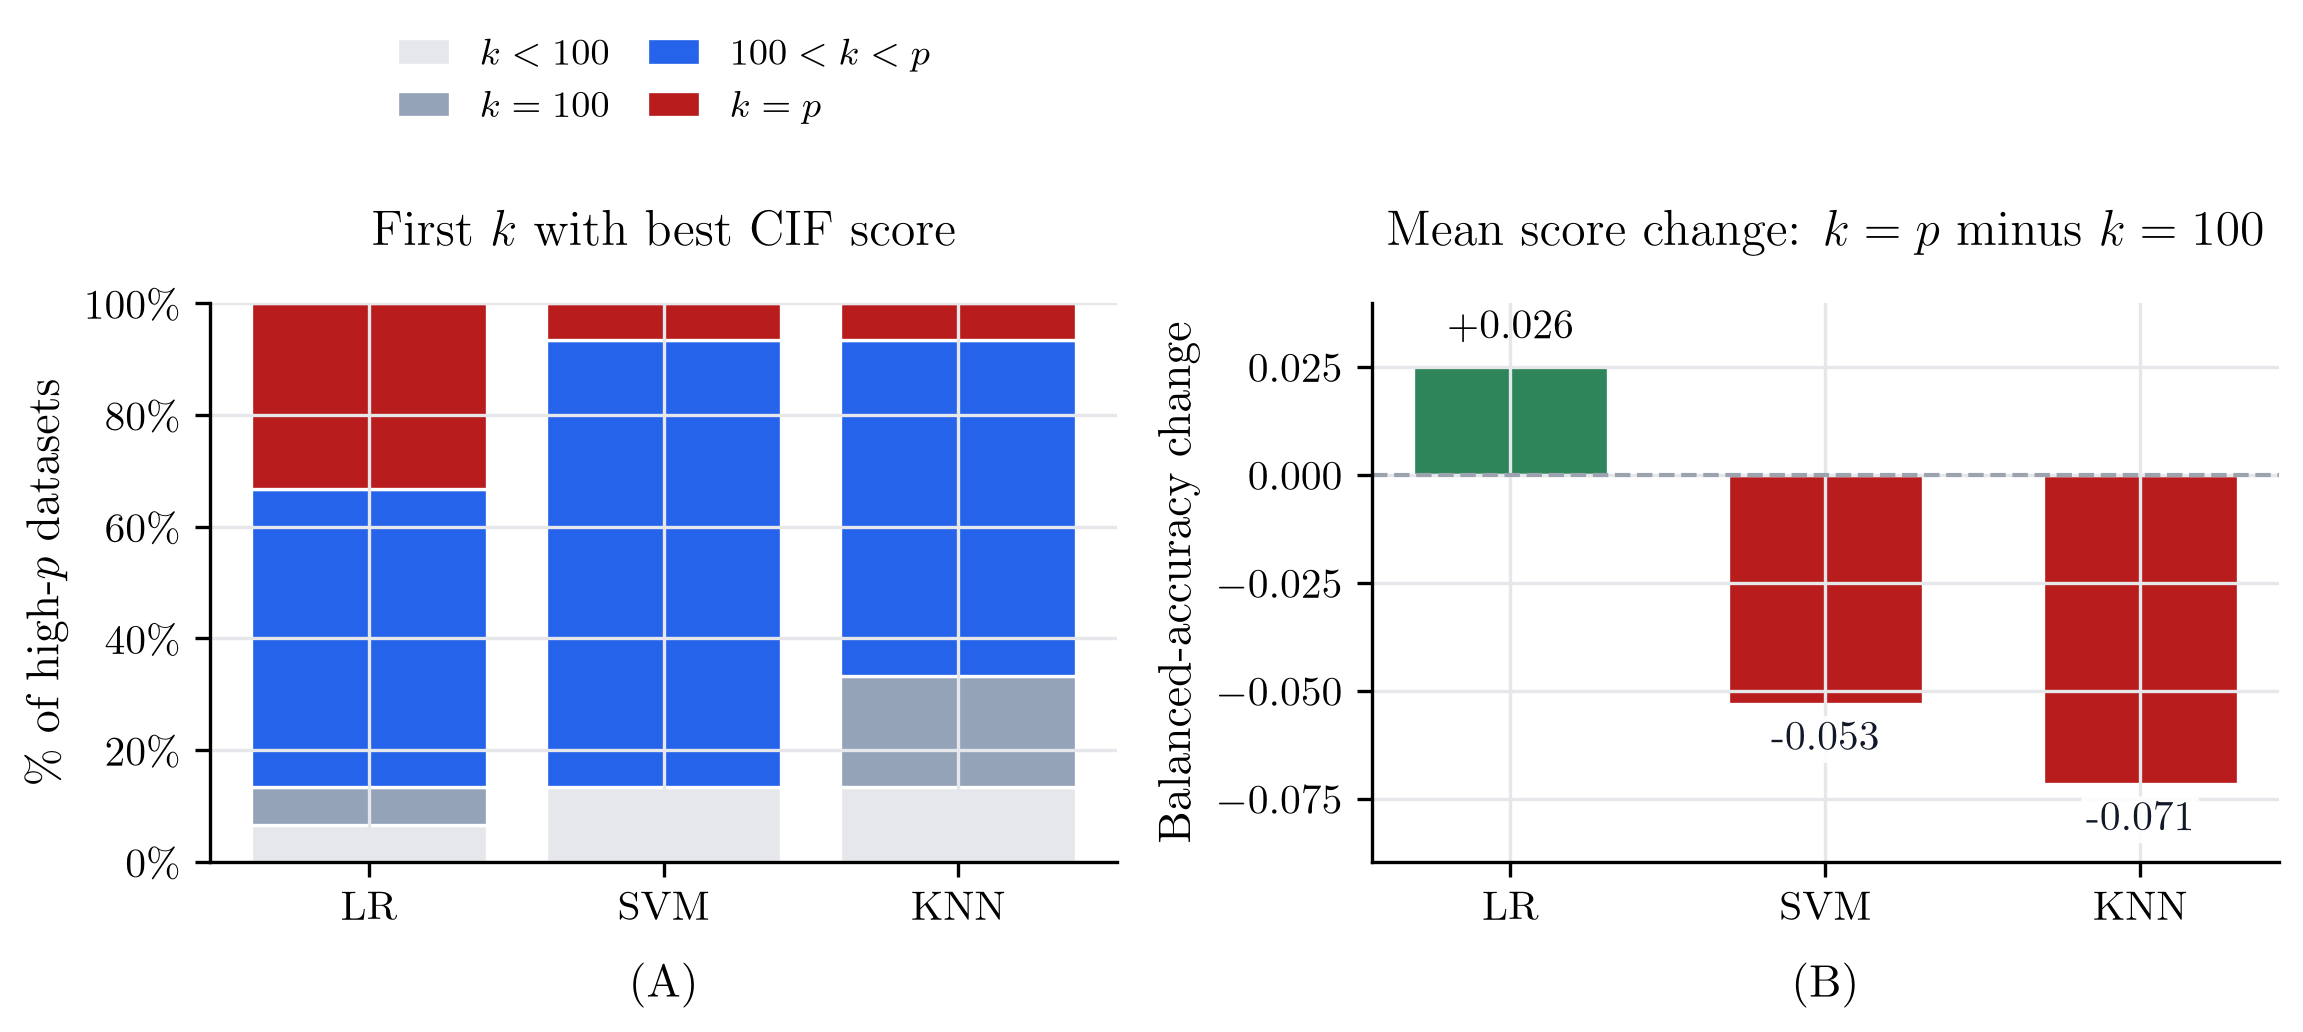
\includegraphics[width=0.84\linewidth]{figures/high_p_boundary_summary.png}
  \caption{Where CIF's classification scores peak as $k$ increases, by
  downstream learner. (A) shows, for each learner, the percentage of 15
  datasets where the first evaluated $k$ attaining the best observed CIF score
  falls below 100, at 100, between 100 and $p$, or at $k=p$. (B) shows the mean
  balanced accuracy change from $k=100$ to $k=p$.}
  \label{fig:high-p-boundary}
\end{figure}

\subsection{Synthetic recovery by \texorpdfstring{$k$}{k}}

\Cref{fig:synthetic-topk-curves} shows synthetic recovery as $k$ grows for
CIT, the forests, and the boosted trees, the curves behind the averages over
$k$ in \cref{tab:synthetic-head}.

\begin{figure}[tb]
  \centering
  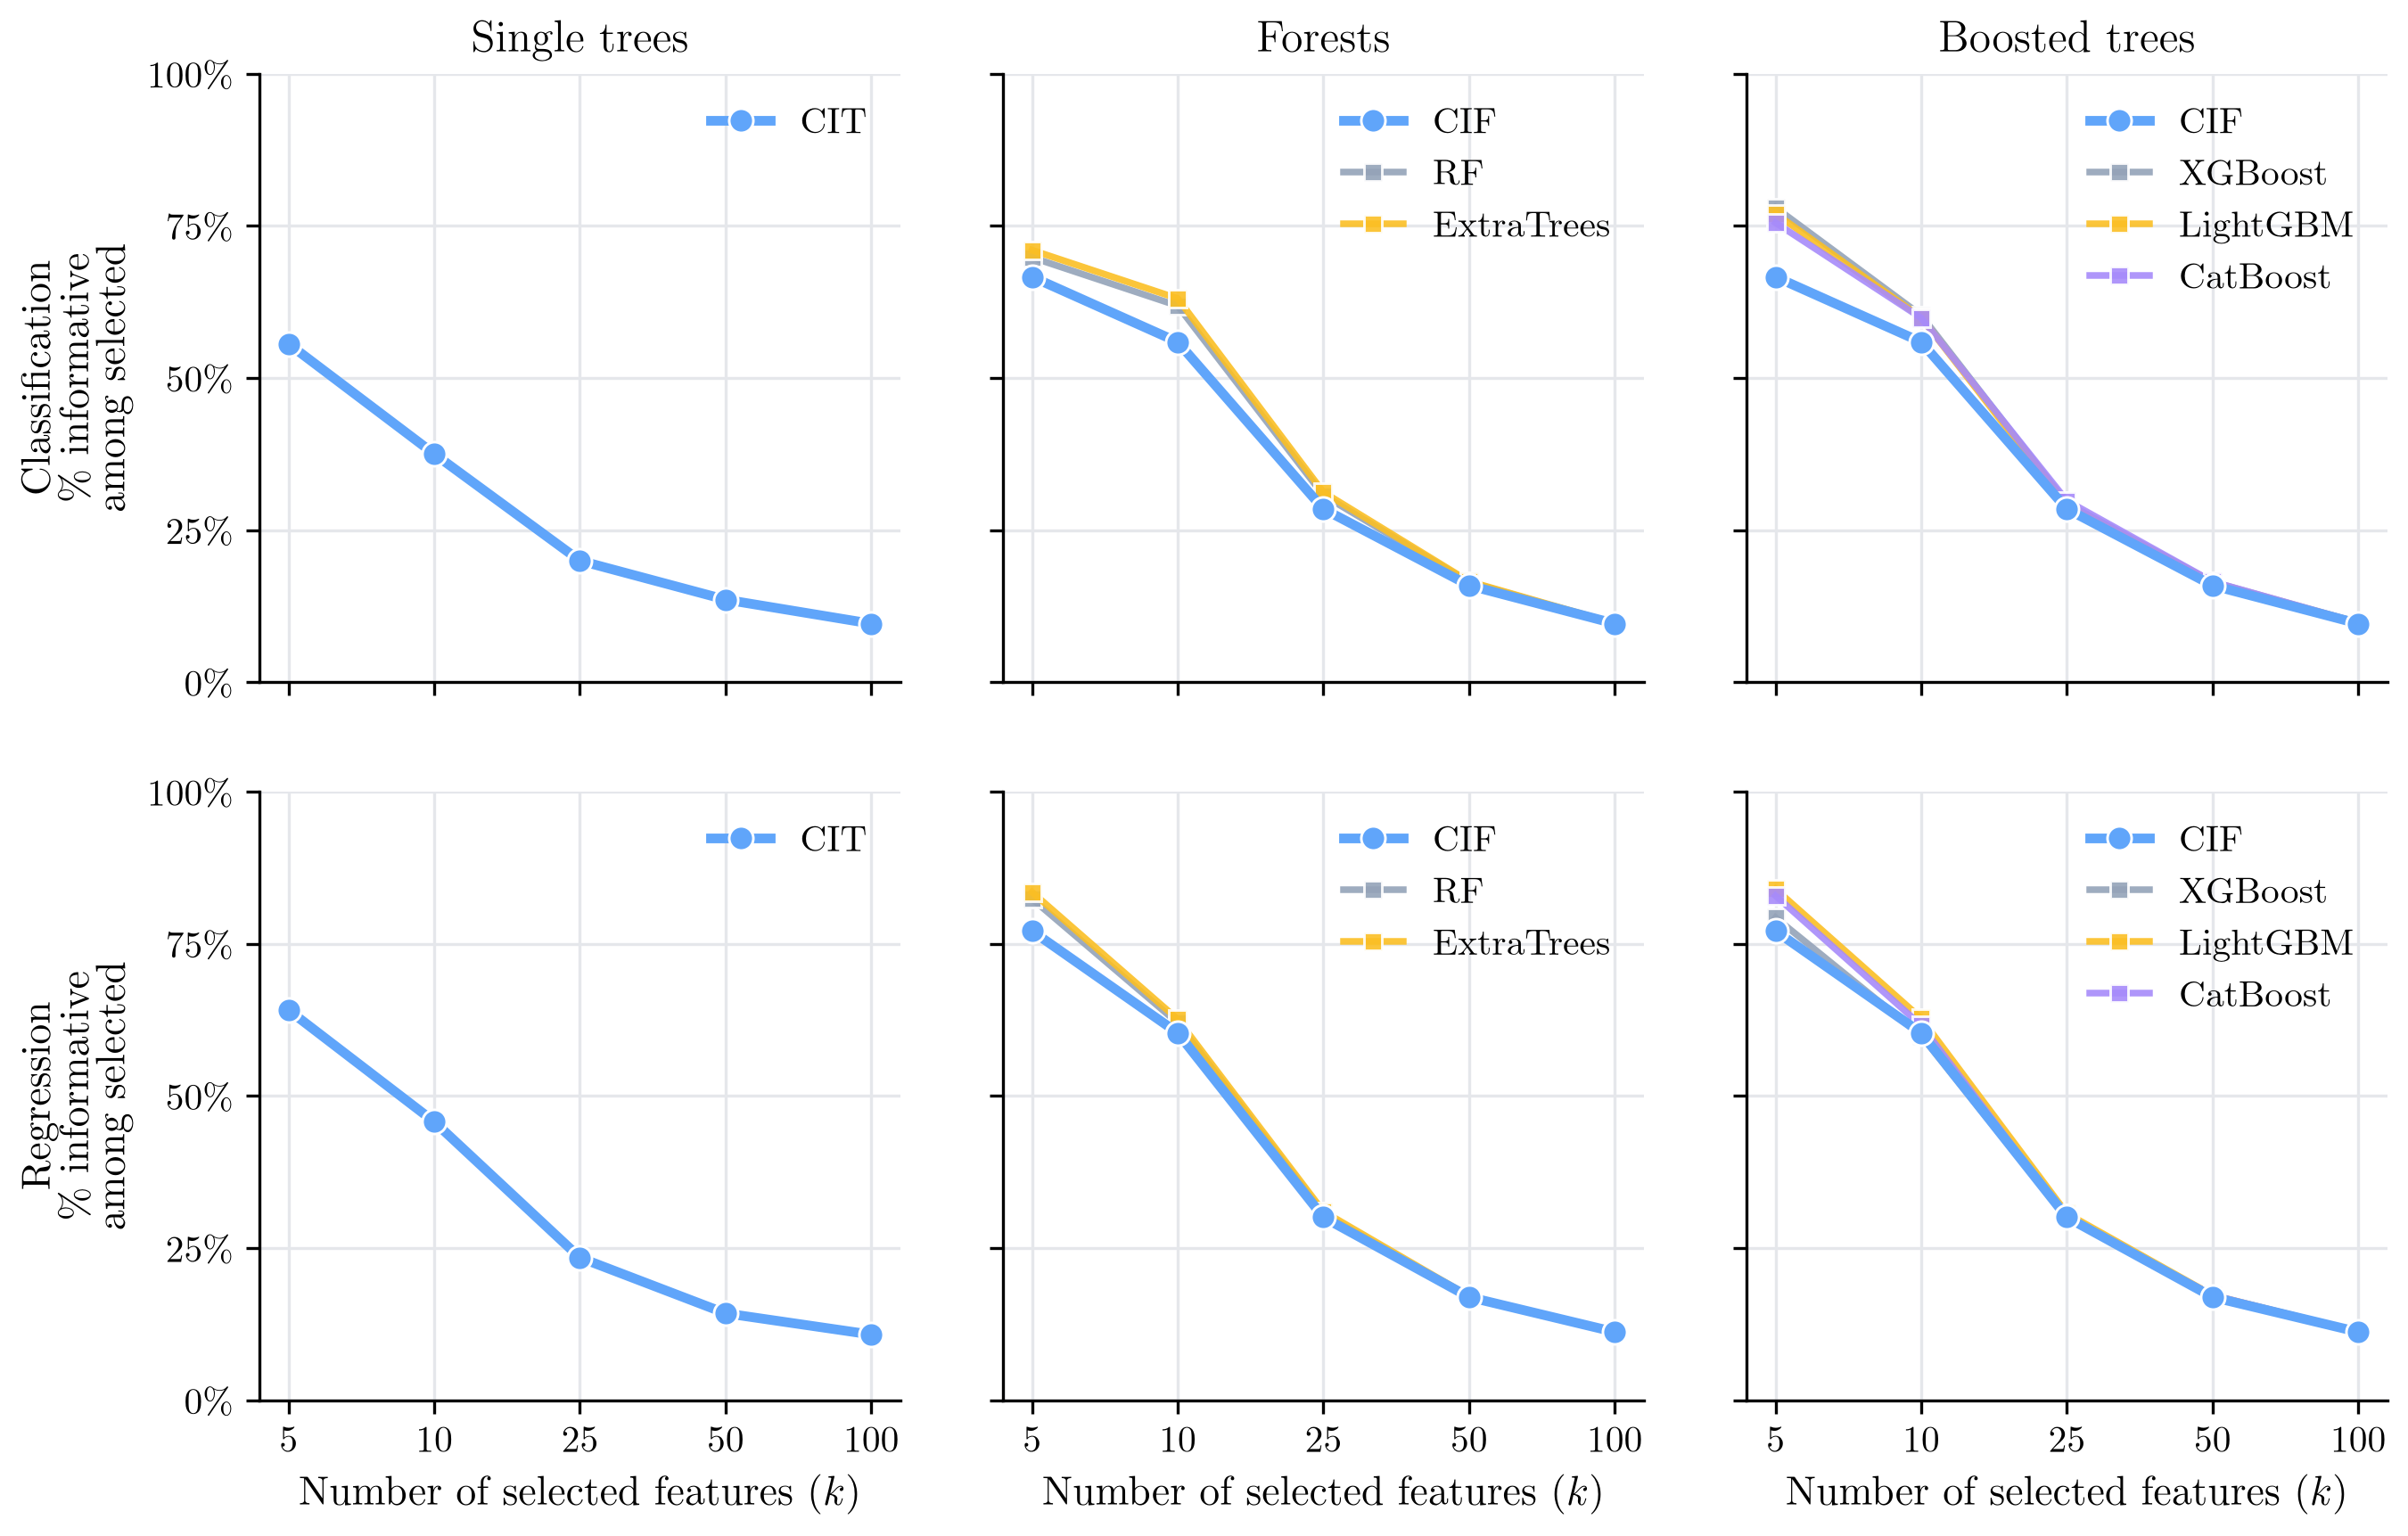
\includegraphics[width=0.84\linewidth]{figures/synthetic_topk_focus_curves.png}
  \caption{Synthetic top-$k$ recovery curves. Columns show CIT alone, then CIF
  against the forests and against the boosted trees; rows show classification
  and regression. Each
  value is the percentage of selected features that are truly informative.}
  \label{fig:synthetic-topk-curves}
\end{figure}

\subsection{Feature use in sampled forests}
\label{app:candidate-availability}

\Cref{sec:mechanism} measures feature use by comparing CIF with CIF-all, which
keeps feature muting and the other tree settings unchanged while removing
feature subsampling. \Cref{fig:candidate-forest-counts} shows how many trees
use each feature in the design with two informative features among 1,000.
CIF-all splits on one informative feature in every tree and on no
uninformative feature, while CIF, RF, and ExtraTrees spread their splits over
the uninformative columns; in that design CIF uses an informative feature in
9.0\% of splits, RF in 2.7\%, ExtraTrees in 2.0\%, and CIF-all in 100.0\%.
Across $p \in \{100,500,1{,}000\}$ with 1,000 trees per fit, evaluating all
nonconstant features raises the share of splits on informative features most
in the sparse high-$p$ classification settings: with two informative features,
CIF uses informative features in 40.0, 12.2, and 9.0\% of splits at $p=100$,
500, and 1,000, against 100.0, 90.2, and 100.0\% for CIF-all. Regression shows a
similar pattern when one or two features are informative, with a smaller
average gain, 42.3\% of splits on informative features for CIF-all against
27.8\% for CIF. The curves by $p$, with the counts of distinct uninformative
features each forest uses, follow in \cref{app:feature-use-dimension}.

\begin{figure}[tb]
  \centering
  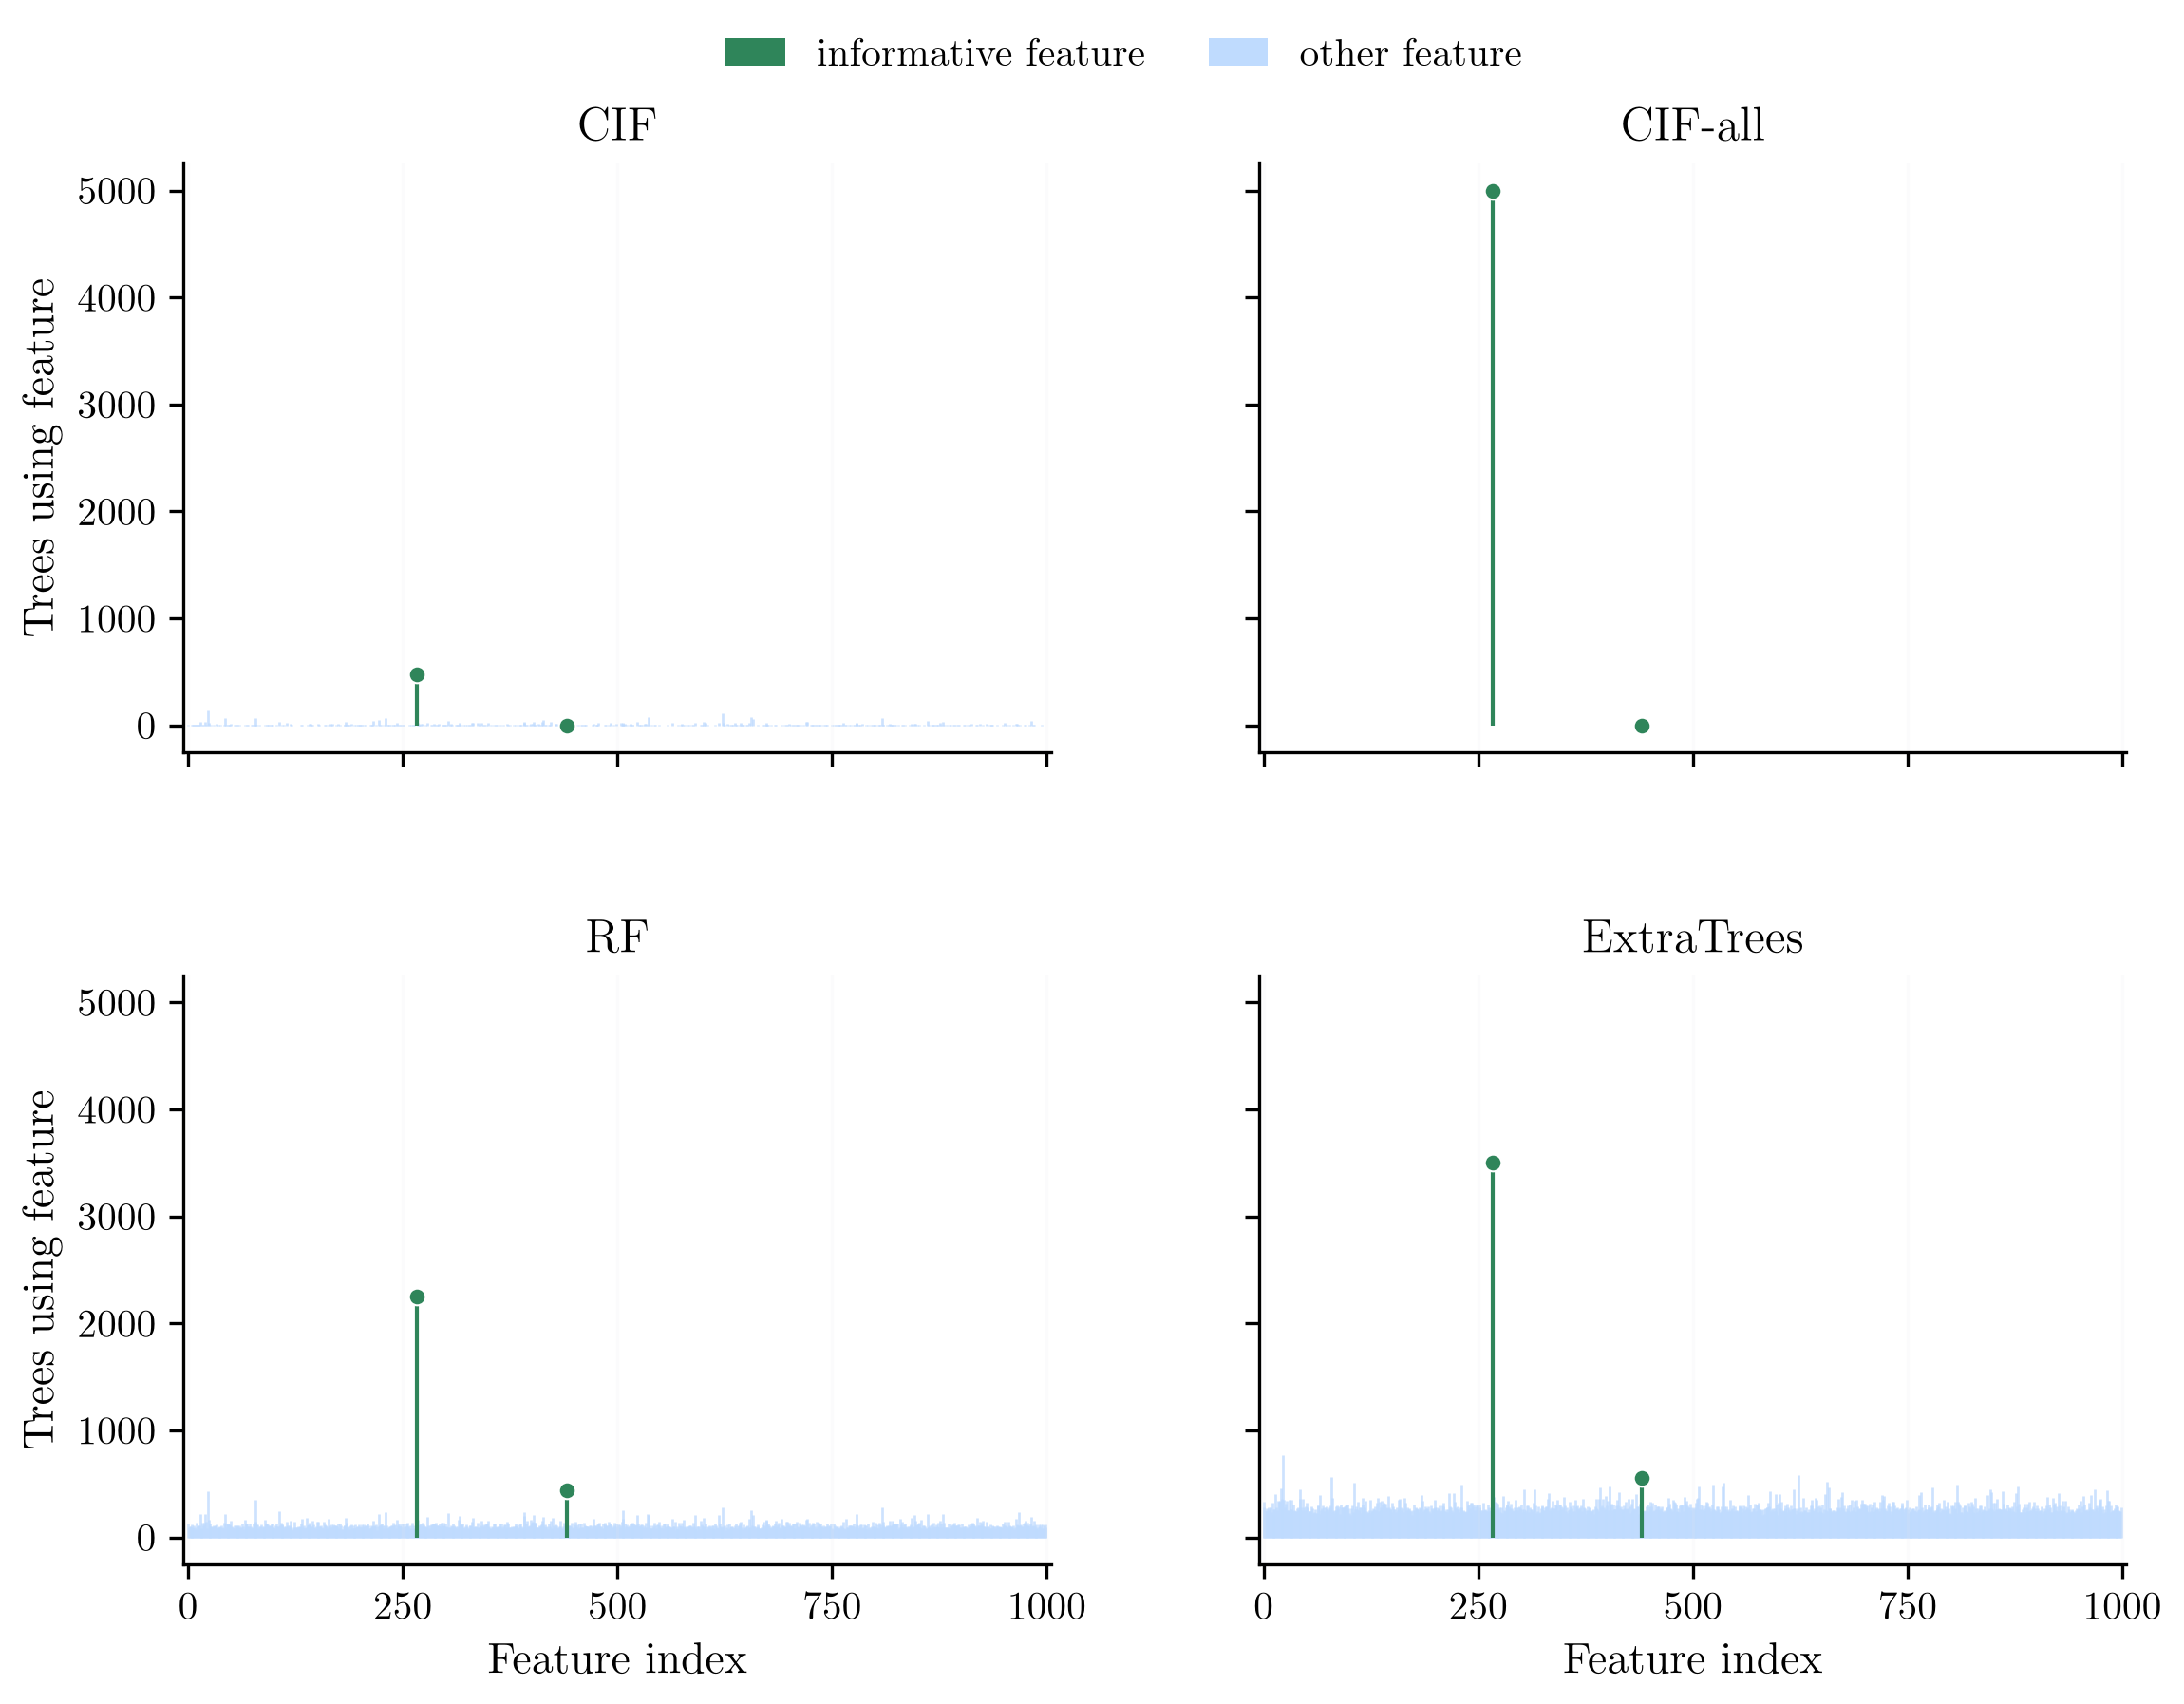
\includegraphics[width=0.84\linewidth]{figures/paper_mechanism_grid_forest_classification_feature_counts_p1000_i2_1000trees.png}
  \caption{Tree-level feature use in one sparse classification forest design
  ($n=250$, $p=1{,}000$, two informative features). Counts are the number of
  trees using each feature in at least one split, pooled over five fits of
  1,000 trees each, so the shared vertical axis runs to 5,000. CIF samples a
  subset of features at each node; CIF-all evaluates all nonconstant
  features.}
  \label{fig:candidate-forest-counts}
\end{figure}

\subsection{Feature use by feature dimension}
\label{app:feature-use-dimension}

\Cref{fig:candidate-dimension-curves} gives the feature-use curves behind
\cref{app:candidate-availability}, for $p \in \{100,500,1{,}000\}$ with 1,000
trees per fit. Each point is the mean over
$n_{\mathrm{informative}} \in \{1,2,5,10\}$, and the capped bar spans the
minimum and maximum over those four sparse settings; the values quoted below
for one, two, or five informative features come from single designs in the same
runs. In classification, evaluating all nonconstant features also narrows the
set of uninformative features used: over the 12 designs CIF-all uses a mean of
93.4 distinct uninformative features against 265.1 for CIF, each counted over
the five pooled fits of a design. With two informative features, CIF-all uses
70, 264, and 439 fewer distinct uninformative features than CIF at $p=100$,
500, and 1,000 (totals over the pooled fits), and with five informative
features the CIF-all minus CIF differences in the share of informative splits
are 25.1, 56.4, and 54.3\%. In regression, CIF-all uses more distinct
uninformative features than CIF, a mean of 528.8 against 367.7. With two
informative features, CIF uses informative features in 39.9, 19.7, and 11.6\%
of regression splits at the three values of $p$, against 58.8, 46.7, and 35.9\%
for CIF-all, and with one informative feature the CIF-all minus CIF
differences are 29.8, 18.9, and 42.1\%.

\begin{figure}[tb]
  \centering
  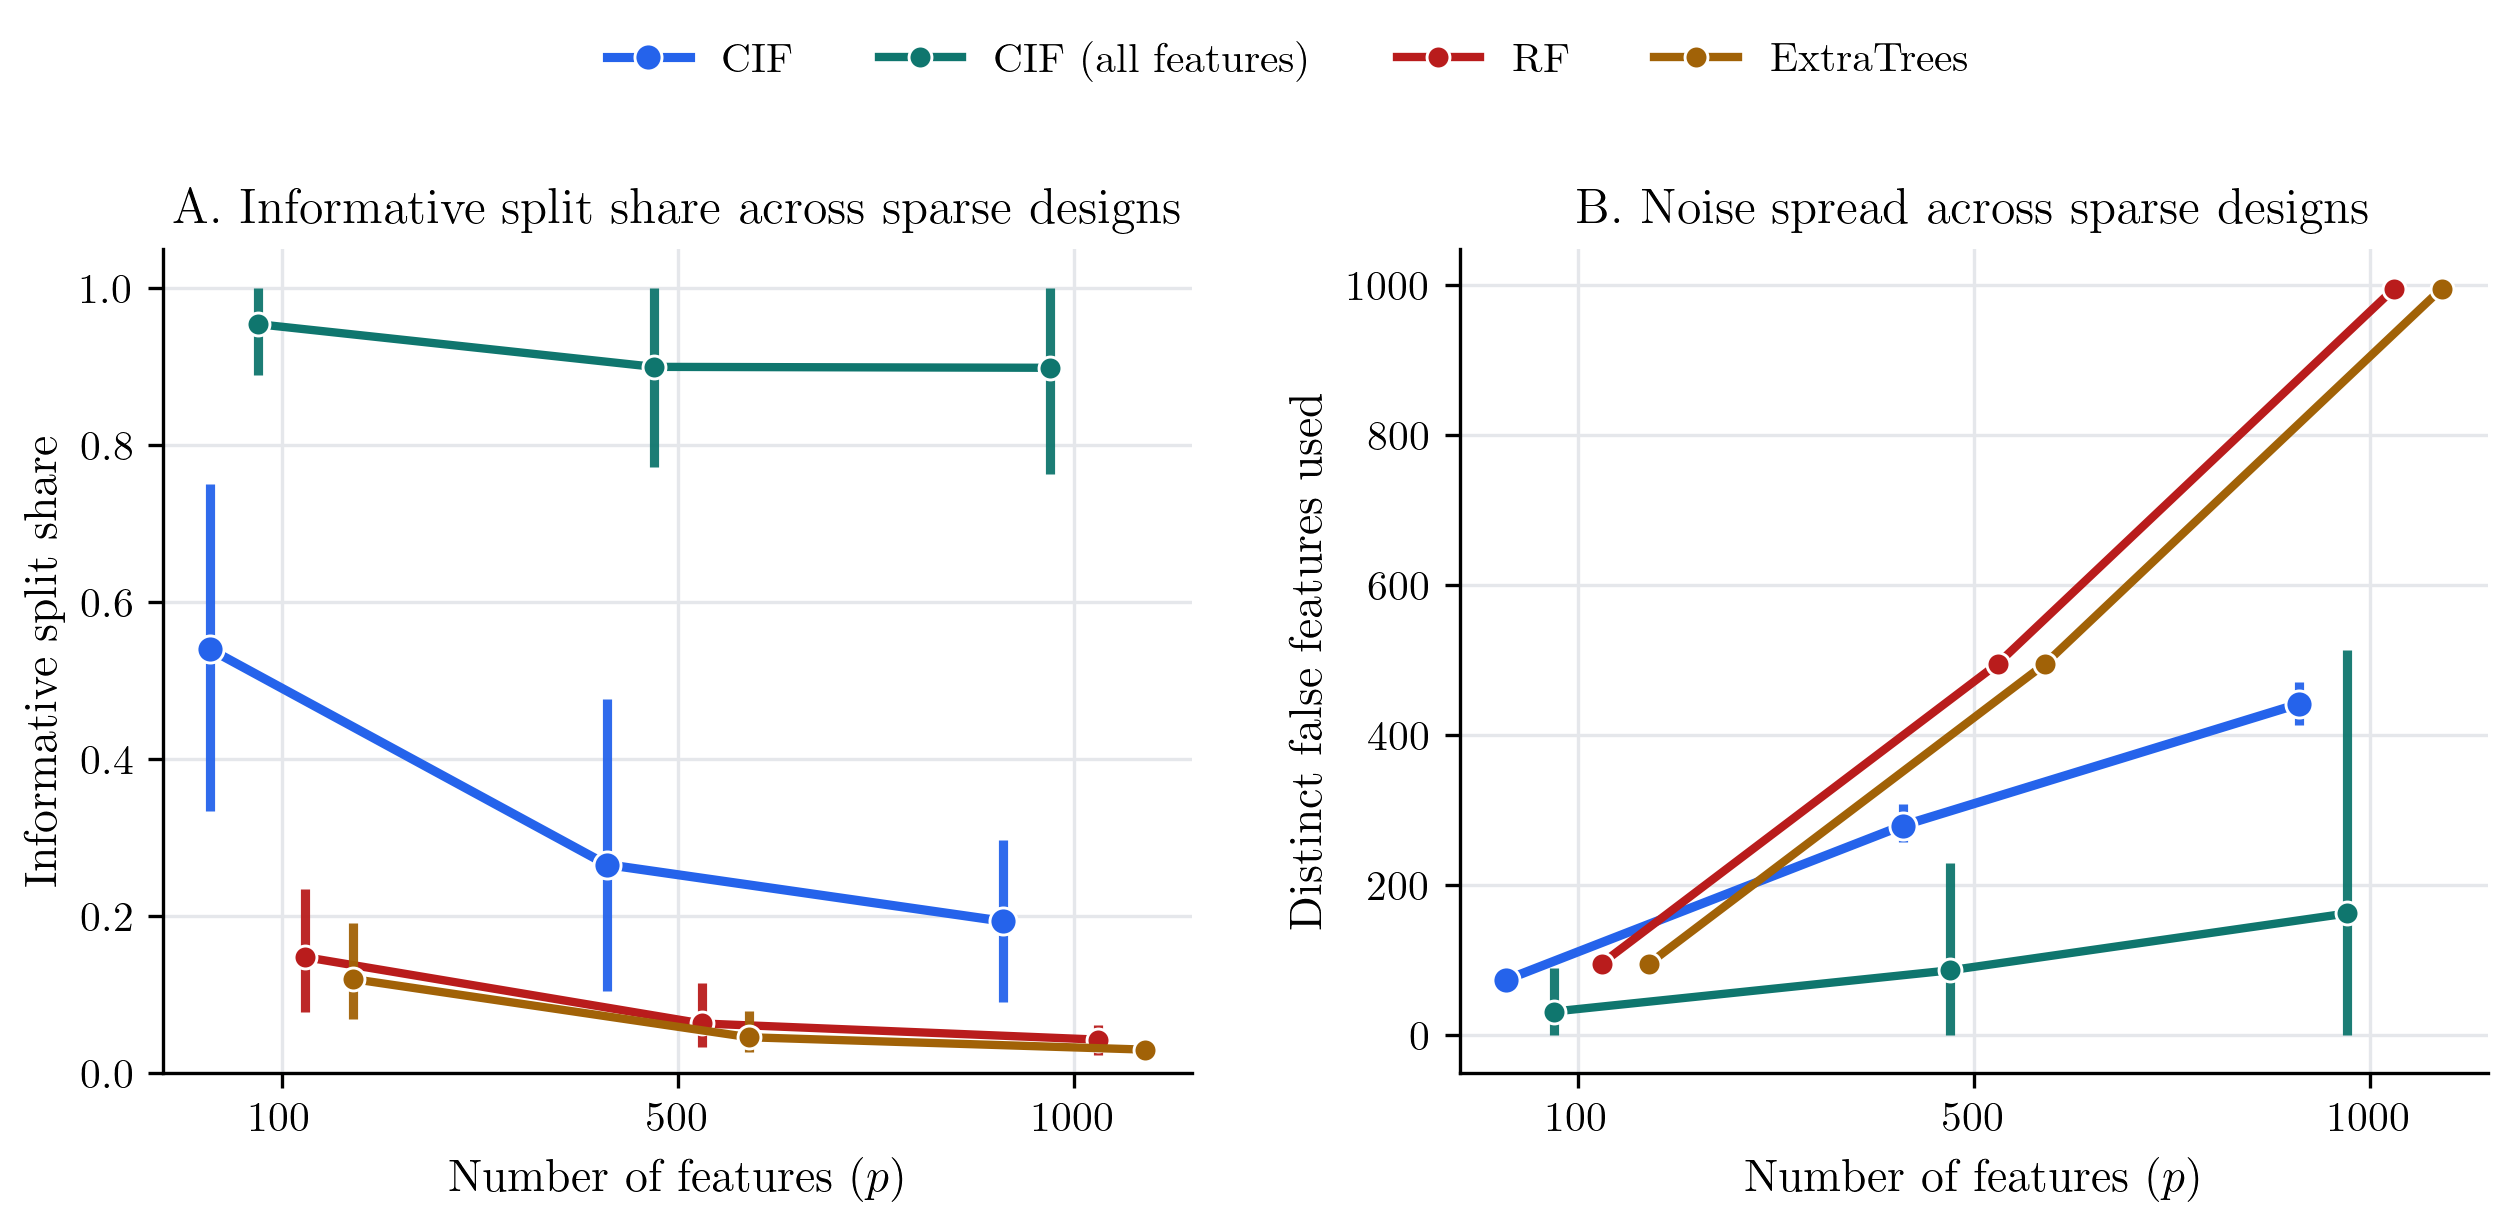
\includegraphics[width=0.88\linewidth]{figures/paper_mechanism_grid_forest_classification_dimension_curves_1000trees.png}\par
  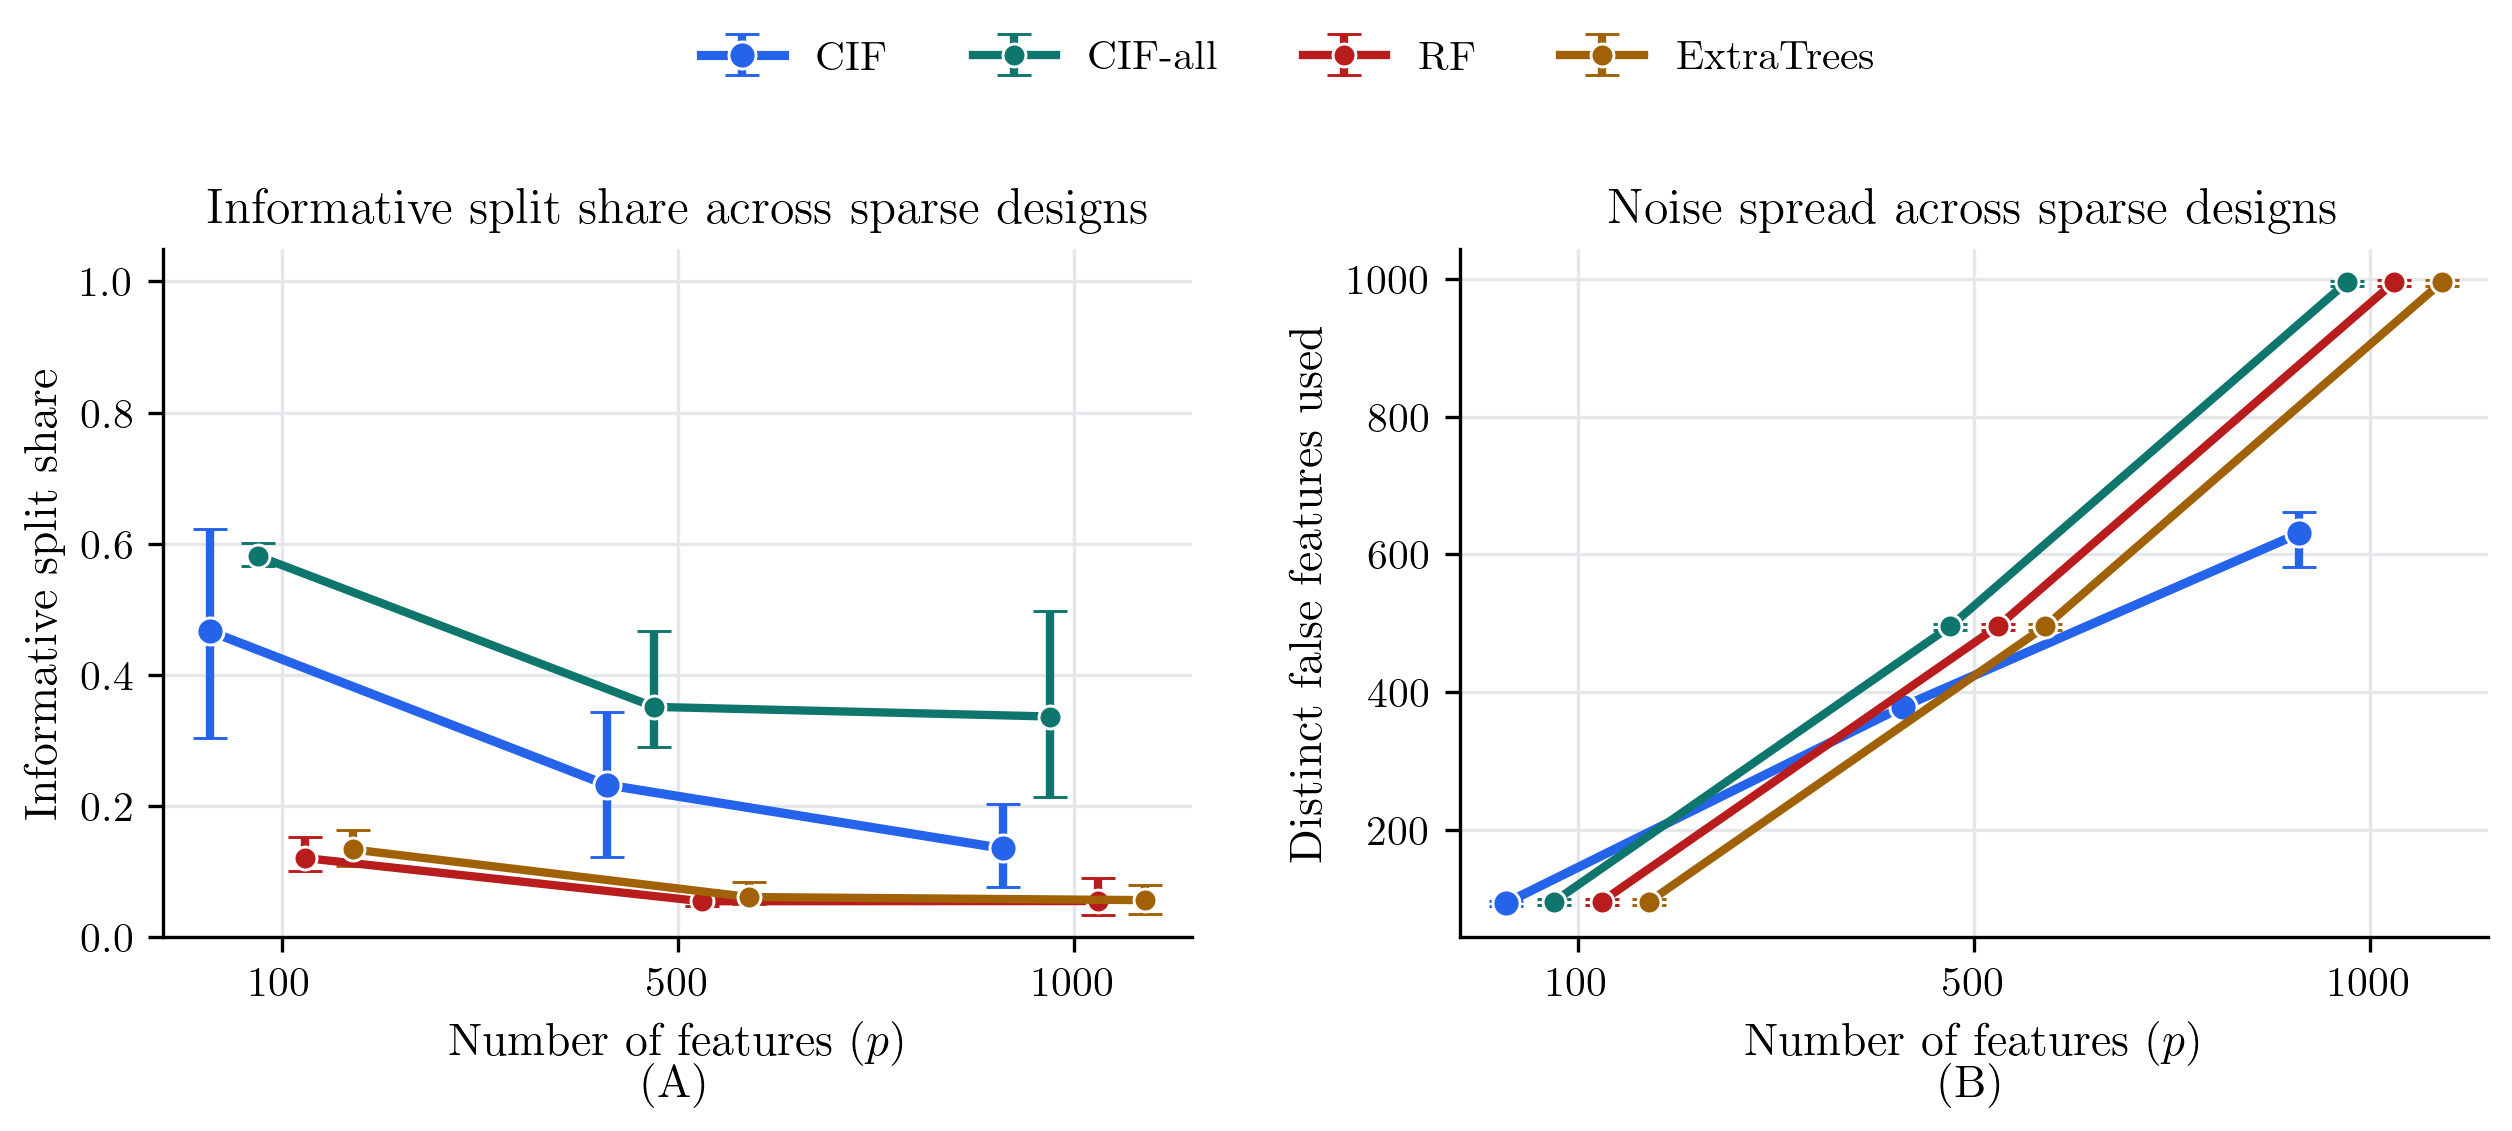
\includegraphics[width=0.88\linewidth]{figures/paper_mechanism_grid_forest_regression_dimension_curves_1000trees.png}
  \caption{Forest feature use by feature dimension $p$, for classification
  (top row) and regression (bottom row), with 1,000 trees per fit. Points are
  means over $n_{\mathrm{informative}} \in \{1,2,5,10\}$; capped bars span the
  minimum and maximum over those four sparse designs. In each row, (A) shows
  the percentage of splits using informative features and (B) the number of
  distinct uninformative features used. CIF samples a subset of features at
  each node; CIF-all evaluates all nonconstant features.}
  \label{fig:candidate-dimension-curves}
  \label{fig:regression-candidate-dimension-curves}
\end{figure}
